

%\documentclass[a4paper]{jarticle}


\section{mgv.rb Graphviz用グラフデータ(.dot)の作成\label{sect:mgv}}
\index{mgv@mgv}

CSV形式のグラフデータを、Graphvizが読み込める.dot形式に変換する。

Takeパッケージに含まれるmpolishingコマンド等では、
グラフの入出力にCSV形式を用いている。
グラフを資料に掲載したり、グラフの規模や密度を目視するには、
グラフを視覚化(画像として描画)する必要がある。

.dot形式に変換することで、
Graphviz(\url{http://www.graphviz.org})のほか
Gephi(\url{http://www.gephi.org})など
グラフ視覚化ソフトウェアに読み込ませることが可能となる。

ただし、Graphvizは比較的小規模なグラフの描画を目的としているため、
頂点数が数百〜数千となると描画時間の面で実用的でなくなる。
大規模グラフの操作・描画にあたってはGephiの使用を推奨する。

\subsection{書式}
\begin{verbatim}
mgv.rb [ni=] [nf=] [nv=] [nr=] [-nl] ei= ef= [ev=] [er=] [-el] [-d] [o=] [--help]
\end{verbatim}

\begin{table}[htbp]
{\small
\begin{tabular}{ll}
\verb|ni=| & : 頂点集合ファイル名 \\
\verb|nf=| & : 頂点ID項目名 \\
\verb|nv=| & : 頂点属性(頂点の大きさ)項目名 \\
\verb|nr=| & : グラフ描画時のノードの拡大率。1から10までの実数値を指定できる。デフォルト値は3 \\
\verb|-nl| & : \verb|nv=|で指定した値をノードの名称に加える \\
\verb|ei=| & : 枝集合ファイル名 \\
\verb|ef=| & : 開始頂点ID項目名,終了頂点ID項目名 \\
\verb|ev=| & : 枝属性(枝の太さ)項目名 \\
\verb|er=| & : グラフ描画時のエッジの拡大率。1から20までの実数値を指定できる。デフォルト値は10 \\
\verb|-el| & : \verb|ev=|で指定した値をエッジの横に表示する \\
\verb|-d|  & : 有向グラフとみなすとき指定する \\
\verb|o=|  & : 出力ファイル名(.dotファイル) \\
\verb|--help| & : ヘルプの表示 \\
\end{tabular} 
}
\end{table} 

入力するグラフデータは、\verb|ei=|パラメータで指定する枝集合のCSVのみでかまわない。
頂点にも属性(大きさ)を与えたい場合は、\verb|ni=|パラメータを用いて
頂点集合のCSVを指定することができる。

\subsubsection*{CSV形式のグラフデータ例}

1行が1本の枝を表し、枝は開始頂点と終了頂点の2項目で表されている。

\begin{Verbatim}[baselinestretch=0.7,frame=single]
node1,node2
A,B
B,C
C,A
C,D
E,D
\end{Verbatim}

\subsubsection*{.dot形式のグラフデータ例}

頂点に関する情報と、枝に関する情報からなる。

\begin{Verbatim}[baselinestretch=0.7,frame=single]
digraph G { 
  edge [dir=none]

    n0 [label="A" height=0.5 width=0.75] 
n1 [label="B" height=0.5 width=0.75] 
n2 [label="C" height=0.5 width=0.75] 
n3 [label="D" height=0.5 width=0.75] 
n4 [label="E" height=0.5 width=0.75] 


    n0 -> n1 [style="setlinewidth(1.0)"]
n1 -> n2 [style="setlinewidth(1.0)"]
n2 -> n0 [style="setlinewidth(1.0)"]
n2 -> n3 [style="setlinewidth(1.0)"]
n4 -> n3 [style="setlinewidth(1.0)"]

}
\end{Verbatim}

\subsubsection*{Graphvizによる描画例}

GraphvizのGUIから対話的に読み込むことができるほか、
Graphvizと一緒にインストールされる\verb|dot|コマンドを使用して
画像ファイル(.pngファイル)に直接変換することもできる。
視覚化したグラフを図\ref{fig:mgv0}に示す。

\begin{Verbatim}[baselinestretch=0.7,frame=single]
$ dot -Tpng rsl1.dot > rsl1.png
$ open rsl1.png
\end{Verbatim}

\begin{figure}[htbp]
\begin{center}
\begin{tabular}{c}

\begin{minipage}{1.0\hsize}
\begin{center}
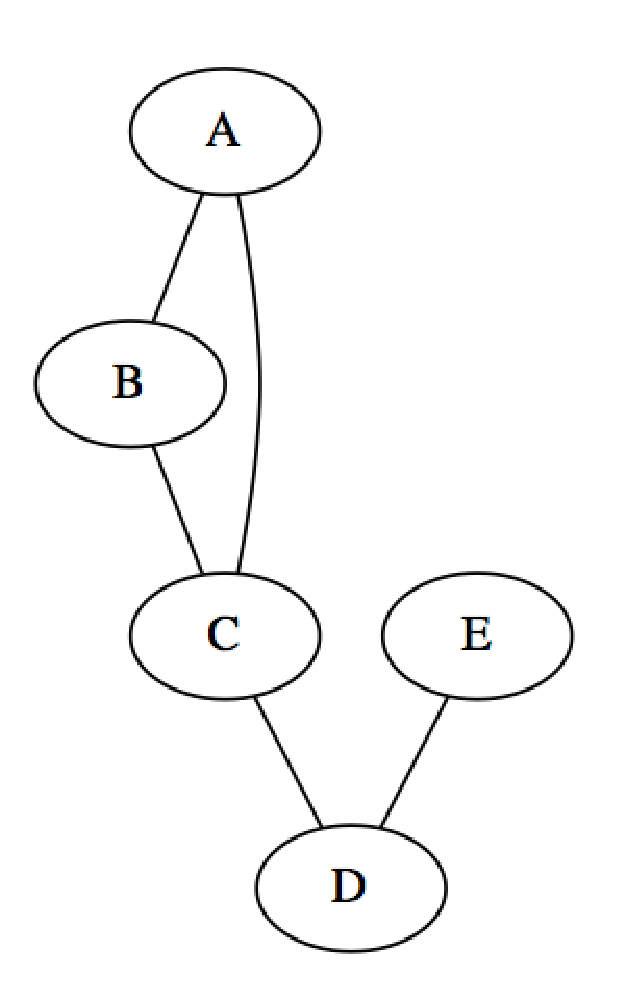
\includegraphics[scale=0.5]{figure/mgv0.eps}
\caption{Graphvizによる描画例\label{fig:mgv0}}
\end{center}
\end{minipage}

\end{tabular}
\end{center}
\end{figure}

\newpage
\subsection{利用例}
\subsubsection*{例1: 基本例}

開始頂点と終了頂点からなる枝集合ファイルのみを与える。


\begin{Verbatim}[baselinestretch=0.7,frame=single]
$ more edge1.csv
node1,node2
A,B
B,C
C,A
C,D
E,D
$ mgv.rb ei=edge1.csv ef=node1,node2 o=rsl1.dot
\end{Verbatim}
\begin{minipage}{1.0\hsize}
\begin{center}
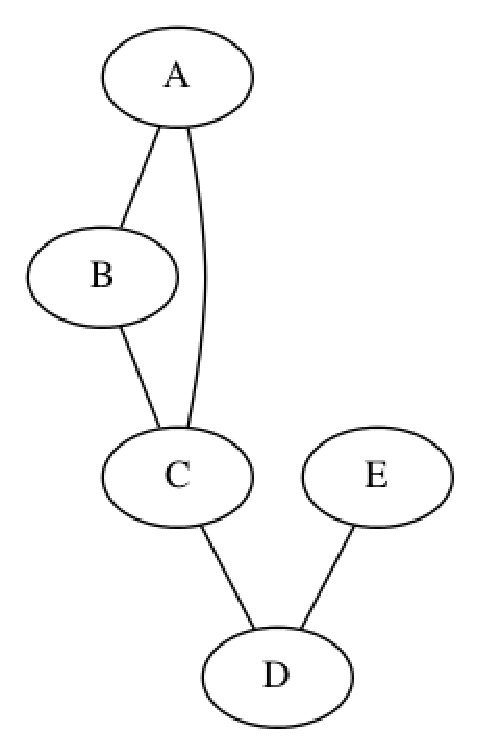
\includegraphics[scale=0.5]{figure/mgv1.eps}
\end{center}
\end{minipage}
\subsubsection*{例2: 枝に属性(太さ)を指定する例}

\verb|ev=|パラメータで\verb|val|項目を属性(太さ)として指定している。
同時に\verb|-el|オプションを付けることで、属性値もグラフに描画される。


\begin{Verbatim}[baselinestretch=0.7,frame=single]
$ more edge2.csv
node1,node2,val
A,B,10
B,C,20
C,A,30
C,D,40
E,D,20
$ mgv.rb ei=edge2.csv ef=node1,node2 ev=val -el o=rsl2.dot
\end{Verbatim}
\begin{minipage}{1.0\hsize}
\begin{center}
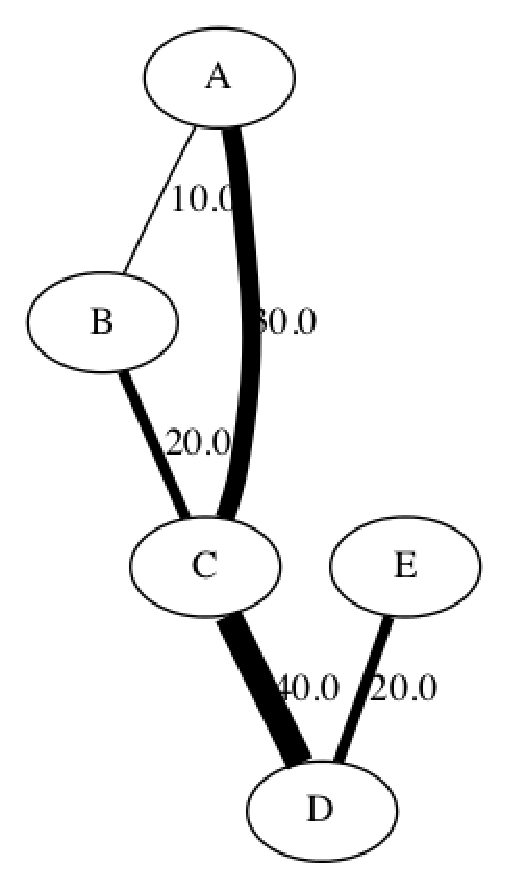
\includegraphics[scale=0.5]{figure/mgv2.eps}
\end{center}
\end{minipage}
\subsubsection*{例3: 頂点に属性(大きさ)を指定する例}

\verb|ni=|パラメータで頂点集合ファイルを指定する。
\verb|nv=|パラメータで、\verb|val|項目を属性(大きさ)として指定している。


\begin{Verbatim}[baselinestretch=0.7,frame=single]
$ more node1.csv
node,val
A,10
B,15
C,8
D,5
E,20
$ more edge1.csv
node1,node2
A,B
B,C
C,A
C,D
E,D
$ mgv.rb ei=edge1.csv ef=node1,node2 ni=node1.csv nf=node nv=val o=rsl3.dot
\end{Verbatim}
\begin{minipage}{1.0\hsize}
\begin{center}
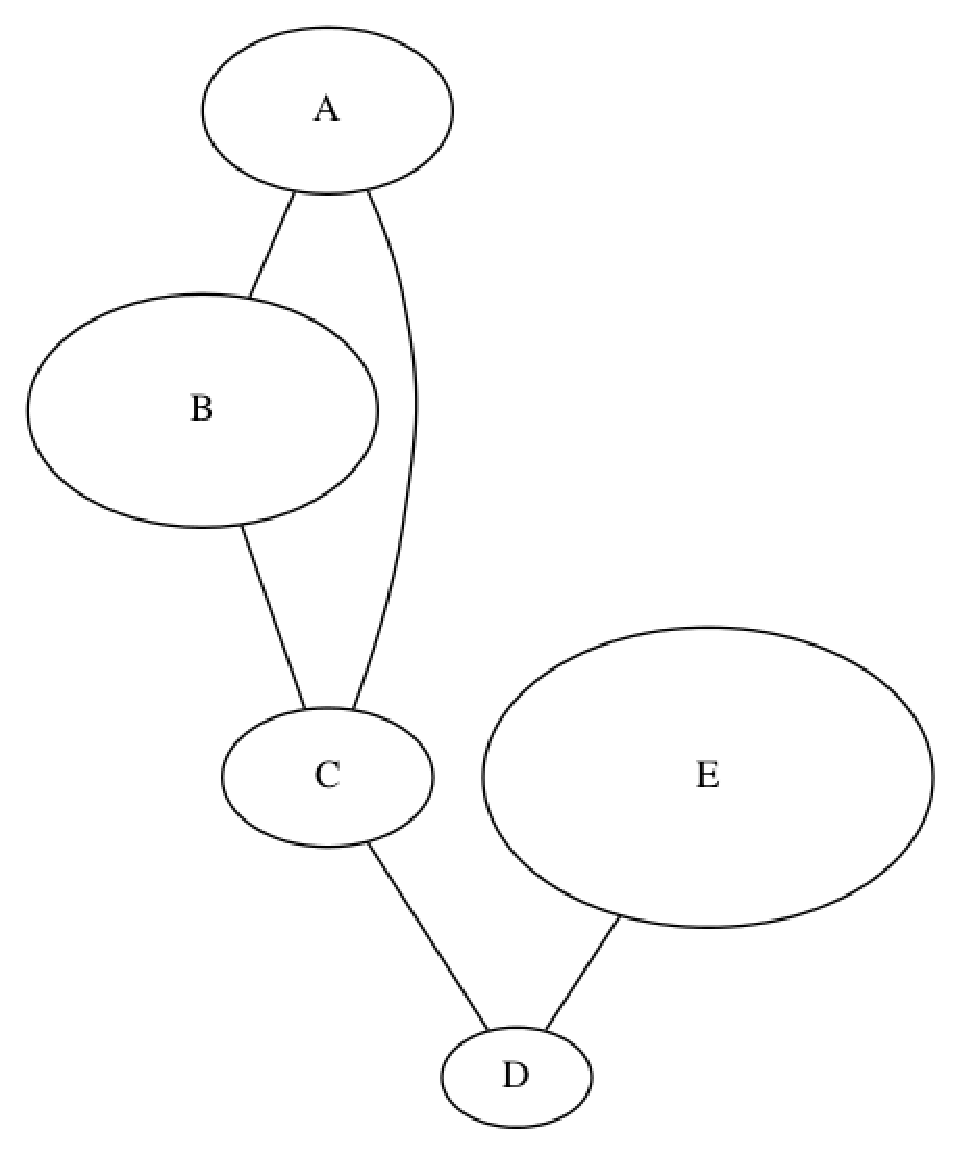
\includegraphics[scale=0.3]{figure/mgv3.eps}
\end{center}
\end{minipage}
\subsubsection*{例4: 頂点に属性(大きさ)と拡大率を指定する例}

\verb|nr=|パラメータで、ノードの拡大率を指定している。


\begin{Verbatim}[baselinestretch=0.7,frame=single]
$ more node1.csv
node,val
A,10
B,15
C,8
D,5
E,20
$ more edge1.csv
node1,node2
A,B
B,C
C,A
C,D
E,D
$ mgv.rb ei=edge1.csv ef=node1,node2 ni=node1.csv nf=node nv=val nr=5 o=rsl4.dot
\end{Verbatim}
\begin{minipage}{1.0\hsize}
\begin{center}
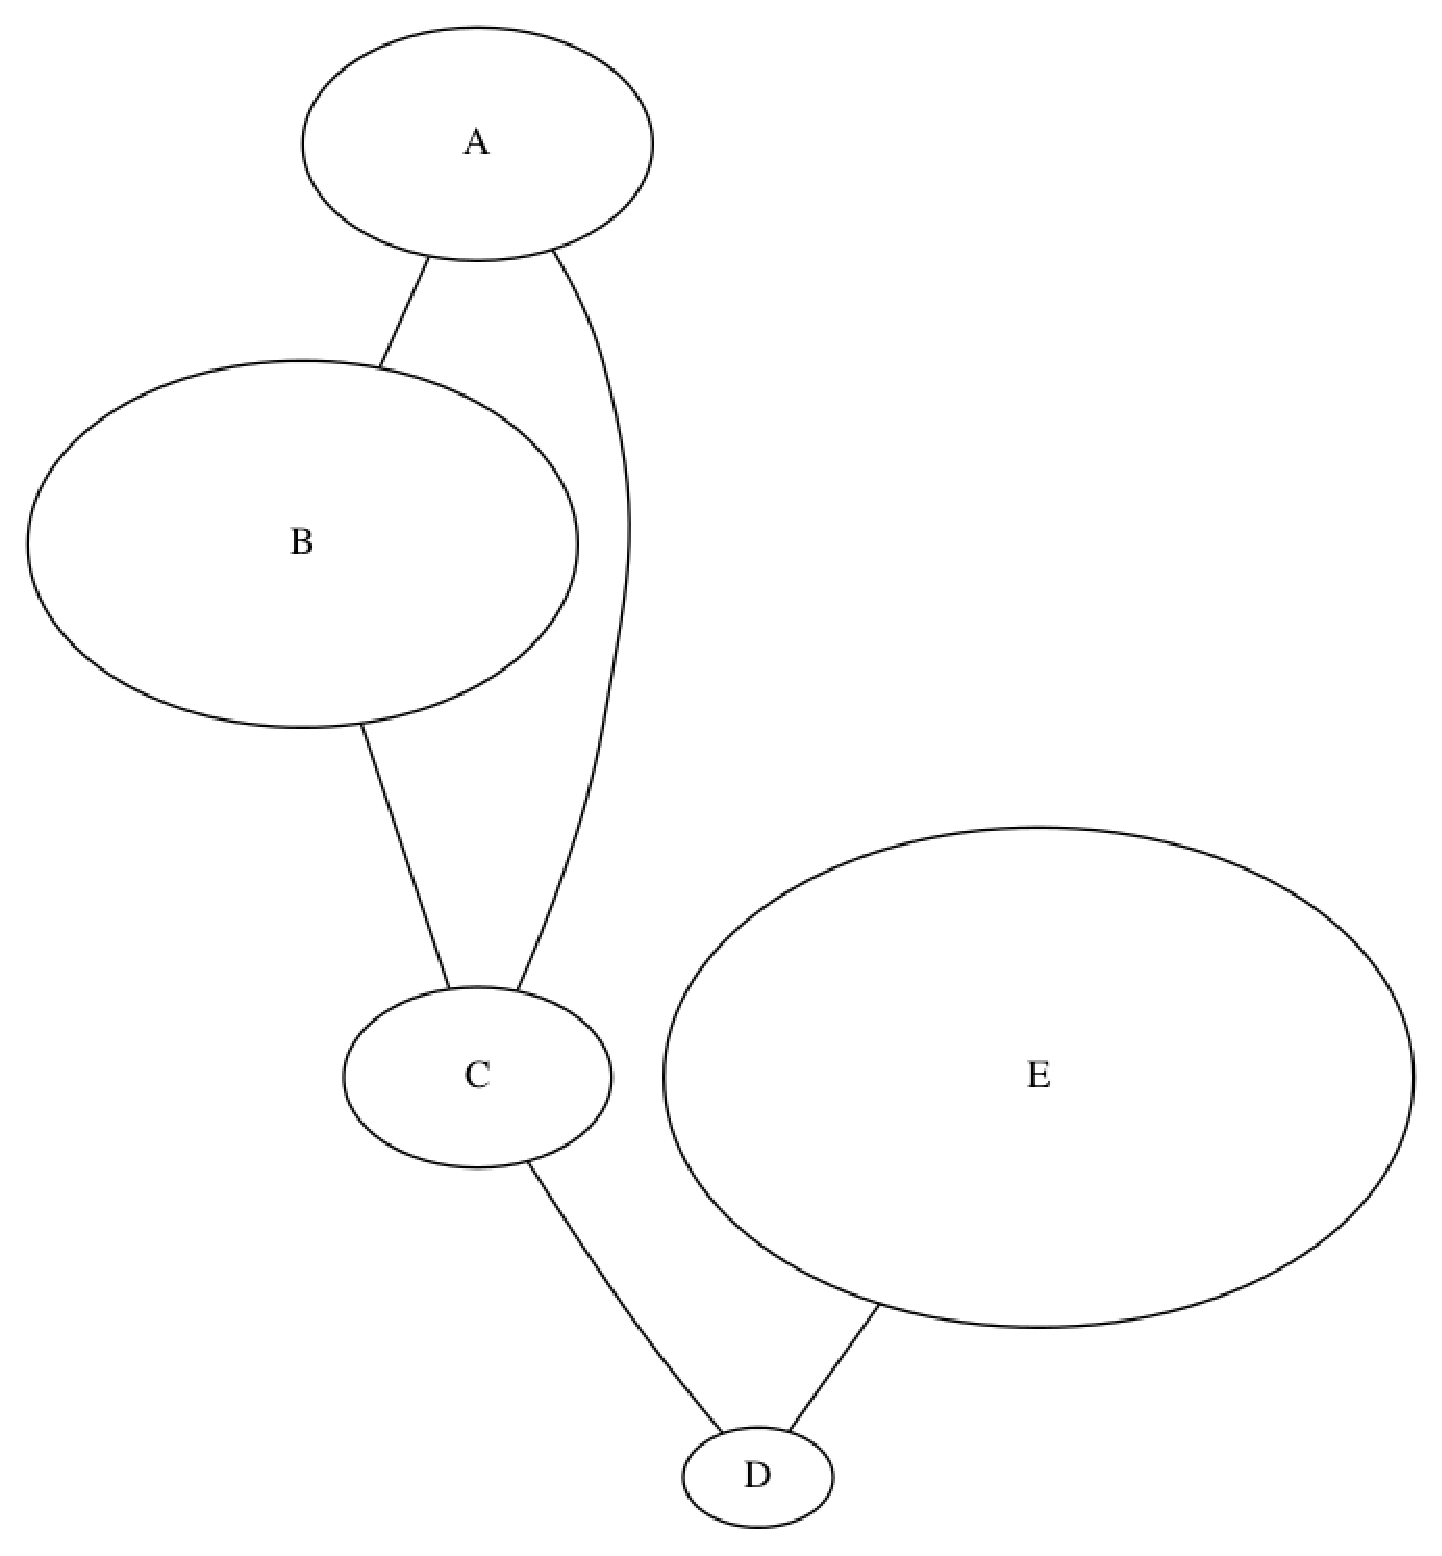
\includegraphics[scale=0.3]{figure/mgv4.eps}
\end{center}
\end{minipage}


%\end{document}

